\chapter{SGANs approximates Jensen–Shannon Divergence}
\label{apx:JSD}
Kullback-Leibler (KL) divergence, by definition is stated as follows
\begin{equation*}
  D_{KL}(p || q) = \int_xp(x)log\left(\frac{p(x)}{q(x)}\right)dx. 
\end{equation*}

Jensen-Shannon (JS) divergence is defined using KL divergence is stated as follows
way
\begin{equation*}
D_{JS}(p || q) = \frac{1}{2}\left(D_{KL}\left(p || \frac{p+q}{2}\right) + D_{KL}\left(q || \frac{p+q}{2}\right)\right).
\end{equation*}


The SGANs loss function, using continuous expectation definition, is stated as follows
\begin{equation*}
  \begin{split}
    \mathcal{L}(G, D) & =  \mathbb{E}_{x \sim p_t(x)}[\log{D(x)}] +  \mathbb{E}_{x \sim p_g(x)}[\log{1 - D(x)}] \\
    & = \int_x(p_t(x)\log{(D(x))} + p_g(x)\log{(1-D(x))})dx \\
    & = \int_xf(x)dx.
  \end{split}
\end{equation*}

First, to find the optimal discriminator $D^*$, we find the maximum of the
function $f(x)$.

\begin{equation*}
\begin{split}
  \frac{df(x)}{dx} & = \frac{p_t(x)}{\ln{10} * D^*(x)} - \frac{p_g(x)}{\ln{10} * (1-D^*(x))} = 0 \Rightarrow \\
  D^*(x) & = \frac{p_t(x)}{p_t(x) + p_g(x)}
\end{split}
\end{equation*}
So the loss function for $D^*(x)$ takes the form
\begin{equation}
  \mathcal{L}(G, D^*) = \int_x(p_t(x)\log{\left(\frac{p_t(x)}{p_t(x) + p_g(x)}\right)} + p_g(x)\log{\left(\frac{p_g(x)}{p_t(x) + p_g(x)}\right)}dx.
  \label{eq:sgan_optimal_disc}
\end{equation}
For the optimal generator $G*$, the probabilities of predicting generated and
target data are equal, i.e. $p_t=p_g$, and the loss function becomes constant
\begin{equation}
\mathcal{L}(G^*, D^*) = -log{4}.
\label{eq:sgan_optimal_gen_disc}
\end{equation}
Now, we can rewrite Equation \ref{eq:sgan_optimal_disc} using the definition of KL
divergence
\begin{equation*}
  \begin{split}
    \mathcal{L}(G, D^*) & = D_{KL}(p_t || p_t + p_g) + D_{KL}(p_g || p_t + p_g) \\ 
    & = D_{KL}\left(p_t || \frac{p_t + p_g}{2}\right) - \log{2} + D_{KL}\left(p_g || \frac{p_t + p_g}{2}\right) -\log{2} \\
    & = D_{JS}(p_t || p_g) - log{4}
  \end{split}
\end{equation*}
Using the Equation \ref{eq:sgan_optimal_gen_disc} for optimal loss we see that
\begin{equation*}
  \mathcal{L}(G^*, D^*) = D_{JS}(p_t || p_g) -log{4} =  - log{4}
\end{equation*}
from which we conclude that for optimal case of training the Jensen-Shannon
divergence is $0$ and the distributions $p_t$ and $p_q$ are equal. $\qed$

% If there are several additions you want to add, but they do not fit into the thesis itself, they belong here.

% \section{Detailed Addition}

% Even sections are possible, but usually only used for several elements in, e.g.\ tables, images, etc.
\let\oldclearpage\clearpage
\let\clearpage\relax
\chapter{Circuits}
\section{Generic Ansatz}
\label{apx:sqgans_ansatz}
\begin{figure}[htbp!]
  \begin{tikzcd}
    \qw &  \gate{R_x(\theta_{(x,1)}^{(i)})} & \gate{R_z(\theta_{(z,1)}^{(i)})} &
    \gate[2, disable auto height]{R_{zz}(\theta_{(1,2)}^{(i)})} & \qw & \qw \\
    \qw &  \gate{R_x(\theta_{(x,2)}^{(i)})} & \gate{R_z(\theta_{(z,2)}^{(i)})} &
    \qw & \gate[2, disable auto height]{R_{zz}(\theta_{(2,3)}^{(i)})} & \qw \\
    \qw &  \gate{R_x(\theta_{(x,3)}^{(i)})} & \gate{R_z(\theta_{(z,3)}^{(i)})} &
    \gate[2, disable auto height]{R_{zz}(\theta_{(3,4)}^{(i)})} & \qw  & \qw \\ 
    \qw &  \gate{R_x(\theta_{(x,4)}^{(i)})} & \gate{R_z(\theta_{(z,4)}^{(i)})} &
    \qw & \vdots \\
     & \vdots & \vdots & \vdots & \vdots & \\
    \qw &  \gate{R_x(\theta_{(x,w-2)}^{(i)})} & \gate{R_z(\theta_{(z,w-2)}^{(i)})} &
    \gate[2, disable auto height]{R_{zz}(\theta_{(w-2,w-1)}^{(i)})} & \vdots \\ 
    \qw &  \gate{R_x(\theta_{(x,w-1)}^{(i)})} & \gate{R_z(\theta_{(z,w-2)}^{(i)})} &
    \vdots & \gate[2, disable auto height]{R_{zz}(\theta_{(w-1,w)}^{(i)})} & \qw \\
    \qw & \gate{R_x(\theta_{(x,w)}^{(i)})} & \gate{R_z(\theta_{(z,w)}^{(i)})} &
    \qw & \qw  & \qw
  \end{tikzcd}
  \caption{Single layer of the generic ansatz used for generator and
    discriminator circuits \cite{Dallaire_Demers_2018}. Circuit parametrized by
    vector $\theta$, where $i$ denotes the layer number and $w$ denotes the
    width of the circuit.
  }
  \label{fig:phase_circuit_apx}
\end{figure}
\section{Topological Phase Transition Ansatz}
This circuit was used by Smith et al. \cite{smith2020crossing} to study
transitions between different states of matter. It is essentially a matrix
product state (MPS) stated in the quantum circuit form.
\label{apx:topological_phase_transition_ansatz}
\begin{figure}[htbp!]
  \begin{tikzcd}
    \lstick{$\ket{0}$} & \gate[2, disable auto height]{U_1(g)} & \qw & \qw & \qw &
    \qw & \qw & \qw \\
    \lstick{$\ket{0}$} & & \gate[2, disable auto height]{U(g)}  & \qw & \qw & \qw & \qw & \qw \\
    \lstick{$\ket{0}$} & \qw & \qw & \gate[2, disable auto height]{U(g)}  & \qw & \qw & \qw & \qw \\
    \lstick{$\ket{0}$} & \qw & \qw & \qw & \qw & \ldots  \\
    \vdots & & & & &\ldots & \gate[2, disable auto height]{U(g)} & \qw \\
    \lstick{$\ket{0}$} & \qw & \qw & \qw & \qw & \qw & \qw & \qw \\
  \end{tikzcd}
  \caption{The topological phase transition circuit studied in \cite{smith2020crossing} }
  \label{fig:phase_circuit_apx}
\end{figure}
\begin{figure}[htbp!]
  \begin{tikzcd}
    \lstick{$\ket{0}$} & \gate{H} & \ctrl{1} & \qw & \qw & \gategroup[2, steps=3,
    style={dashed, fill=blue!20, inner xsep=2pt}, background]{{
        Only for g > 0}}\qw & \ctrl{1} & \qw & \qw \\
    \lstick{$\ket{0}$} & \qw & \targ{} & \gate{Z} & \gate{R_y(\theta_r(g))} & \gate{H} & \targ{} &
    \gate{H} & \qw
  \end{tikzcd}
  \caption{The schema of $U_1$ gate from the circuit in Figure \ref{fig:phase_circuit_apx}}
  \label{fig:phase_circuit_u1}
\end{figure}
\begin{figure}[htbp!]
  \begin{tikzcd}
    \lstick{$\ket{\cdot}$} & \gate{X} & \ctrl{1} & \gate{X} & \qw & \qw & \qw & \ctrl{1} &
     \qw & \gate{X} & \qw & \qw \\
     \lstick{$\ket{0}$} &  \gate{R_y(\theta_w(g))}  & \targ{} &  \gate{X} & \gate{R_y(\theta_w(g))} & \gate{X} &  \gate{R_y(\theta_v(g))}
     & \targ{} & \gate{X} & \gate{R_y(\theta_v(g))} & \gate{X} & \qw
  \end{tikzcd}
  \caption{The schema of $U$ gate from the circuit in Figure \ref{fig:phase_circuit_apx}}
  \label{fig:phase_circuit_u}
\end{figure}

Where
\begin{equation*}
  \begin{split}
    R_y(\theta) & = \begin{pmatrix}
      \cos{\frac{\theta}{2}} & -\sin{\frac{\theta}{2}} \\
      \sin{\frac{\theta}{2}} & \cos{\frac{\theta}{2}} 
    \end{pmatrix}, \\
    \theta_w(g) & = \arccos{\frac{sign(g)\sqrt{|g|}}{\sqrt{1+|g|}}},\ \theta_w \in [0, \pi], \\
    \theta_v(g) & = \arcsin{\frac{\sqrt{|g|}}{\sqrt{1+|g|}}},\ \theta_v \in [-\frac{\pi}{2}, \frac{\pi}{2}], \\
    \theta_r(g) & = 2\arcsin{\frac{1}{\sqrt{1+|g|}}},\ \theta_r \in [-\pi, \pi].
  \end{split}
\end{equation*}

\section{Butterfly Ansatz}
\label{apx:butterfly_ansatz}
\begin{figure}[htbp!]
\begin{tikzcd}
\lstick{$\ket{0}$} & \gate{R_x(\theta_{(1,1)})} & \ctrl{1} &
\gate{R_x(\theta_{(3,1)})} & \ctrl{2} & \qw & \gate{R_x(\theta_{(5,1)})} & \qw &
\ldots & \rstick[wires=9]{$\ket{\psi}$}\\
\lstick{$\ket{0}$} & \gate{R_x(\theta_{(1,2)})} & \gate{R_x(\theta_{(2,1)})}  &
\gate{R_x(\theta_{(3,2)})} & \qw & \ctrl{2} & \gate{R_x(\theta_{(5,2)})} & \qw &
\ldots & \\ 
\lstick{$\ket{0}$} & \gate{R_x(\theta_{(1,3)})} & \ctrl{1} &
\gate{R_x(\theta_{(3,3)})} & \gate{R_x(\theta{(4,1)})} & \qw & \gate{R_x(\theta_{(5,3)})} & \qw &
\ldots & \\
\lstick{$\ket{0}$} & \gate{R_x(\theta_{(1,4)})} & \gate{R_x(\theta_{(2,2)})}  &
\gate{R_x(\theta_{(3,4)})} & \qw & \gate{R_x(\theta{(4,2)})} & \gate{R_x(\theta_{(5,4)})} & \qw &
\ldots & \\ 
\lstick{$\ket{0}$} & \gate{R_x(\theta_{(1,5)})} & \ctrl{1} &
\gate{R_x(\theta_{(3,5)})} & \ctrl{2} & \qw & \gate{R_x(\theta_{(5,5)})} & \qw &
\ldots & \\ 
\lstick{$\ket{0}$} & \gate{R_x(\theta_{(1,6)})} & \gate{R_x(\theta_{(2,3)})}  &
\gate{R_x(\theta_{(3,6)})} & \qw & \ctrl{2} & \gate{R_x(\theta_{(5,6)})} & \qw &
\ldots & \\ 
\lstick{$\ket{0}$} & \gate{R_x(\theta_{(1,7)})} & \ctrl{1} &
\gate{R_x(\theta_{(3,7)})} & \gate{R_x(\theta{(4,3)})} & \qw & \gate{R_x(\theta_{(5,7)})} & \qw &
\ldots & \\ 
\lstick{$\ket{0}$} & \gate{R_x(\theta_{(1,8)})} & \gate{R_x(\theta_{(2,4)})}  &
\gate{R_x(\theta_{(3,8)})} & \qw & \gate{R_x(\theta{(4,4)})} & \gate{R_x(\theta_{(5,8)})} & \qw &
\ldots & \\
\lstick{$\ket{0}$} & \gate{R_x(\theta_{(1,9)})} & \qw  &
\gate{R_x(\theta_{(3,9)})} & \qw & \qw & \gate{R_x(\theta_{(5,9)})} & \qw &
\ldots & \\
\end{tikzcd}
\caption{The butterfly circuit for 9 qubits. For each $j$-th power of $2$ that the
  width of the circuit exceeds, the next layer is added that consist of $R_x$
  gates on each qubit and controlled $R_x$ gate between $i$-th and $i+2^j$-th qubits (continued below).}
\end{figure}
\begin{figure}[htbp!] \ContinuedFloat
\begin{tikzcd}
  \lstick[wires=9]{$\psi$} & \ldots & \ctrl{4} & \qw & \qw &
  \qw & \gate{R_x(\theta_{(7,1)})} & \ctrl{8} & \qw \\
  & \ldots & \qw & \ctrl{4} & \qw & \qw  &
  \gate{R_x(\theta_{(7,2)})} & \qw & \qw\\
  & \ldots & \qw & \qw & \ctrl{4} & \qw &
  \gate{R_x(\theta_{(7,3)})}  \qw & \qw & \qw\\
  & \ldots & \qw & \qw & \qw & \ctrl{4}  &
  \gate{R_x(\theta_{(7,4)})}  \qw & \qw & \qw\\
  &  \ldots &\gate{R_x(\theta_{(6,1)})} & \qw & \qw & \qw &
  \gate{R_x(\theta_{(7,5)})}  \qw & \qw & \qw\\
  & \ldots & \qw & \gate{R_x(\theta_{(6,2)})}  & \qw & \qw &
  \gate{R_x(\theta_{(7,6)})}  \qw & \qw & \qw\\
  & \ldots & \qw & \qw & \gate{R_x(\theta_{(6,3)})} & \qw &
  \gate{R_x(\theta_{(7,7)})}  \qw & \qw & \qw\\ 
  &  \ldots &\qw & \qw & \qw & \gate{R_x(\theta_{(6,4)})}  &
  \gate{R_x(\theta_{(7,8)})}  \qw & \qw & \qw\\
  & \ldots & \qw & \qw & \qw & \qw &
  \gate{R_x(\theta_{(7,9)})}  & \gate{R_x(\theta_{(8,1)})} & \qw \\
\end{tikzcd}
\caption{The butterfly circuit for 9 qubits. For each $j$-th power of $2$ that the
    width of the circuit exceeds, the next layer is added that consist of $R_x$
    gates on each qubit and controlled $R_x$ gate between $i$-th and $i+2^j$-th qubits }
\end{figure}
\chapter{WQGANs Additional Results}
\label{apx:wqgans_pahse_results}
\begin{figure}[htbp!]
  \captionsetup[subfigure]{labelformat=empty}
  \centering
  \subfloat{
    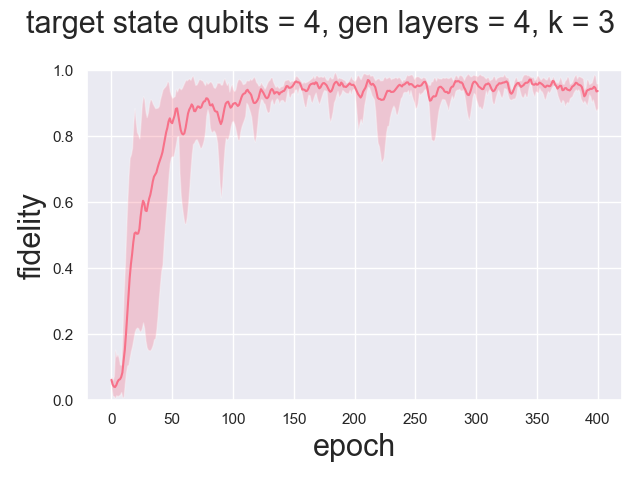
\includegraphics[width=0.3\linewidth]{figures/wqgans_phase_size=4_k=3_gen=4/fidelity.png}
  }
  \subfloat{
    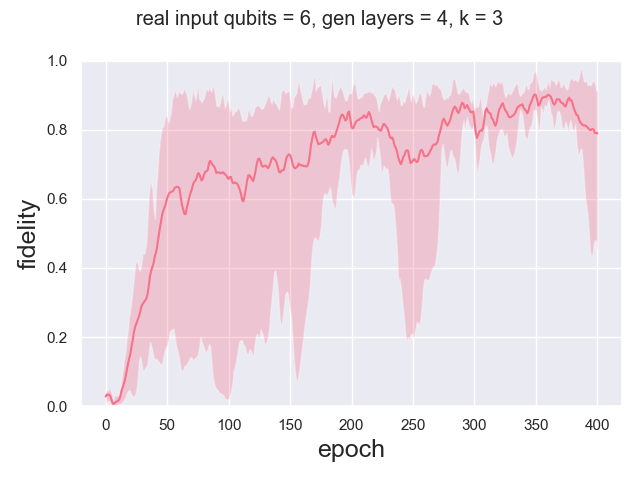
\includegraphics[width=0.3\linewidth]{figures/wqgans_phase_size=6_k=3_gen=4/fidelity.png}
  }
  \subfloat{
    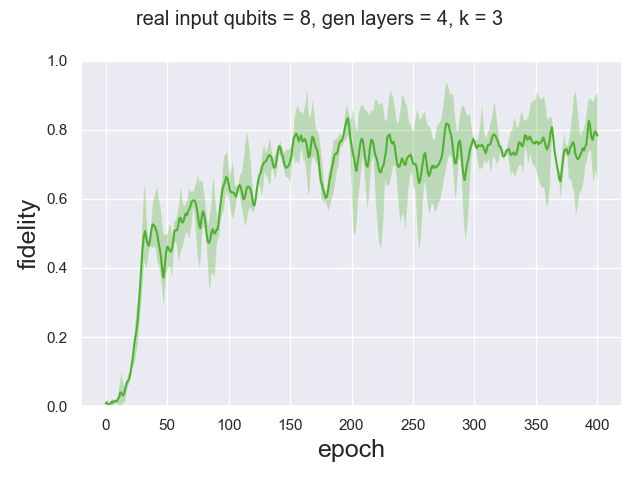
\includegraphics[width=0.3\linewidth]{figures/wqgans_phase_size=8_k=3_gen=4/fidelity.png}
  }

  \subfloat{
    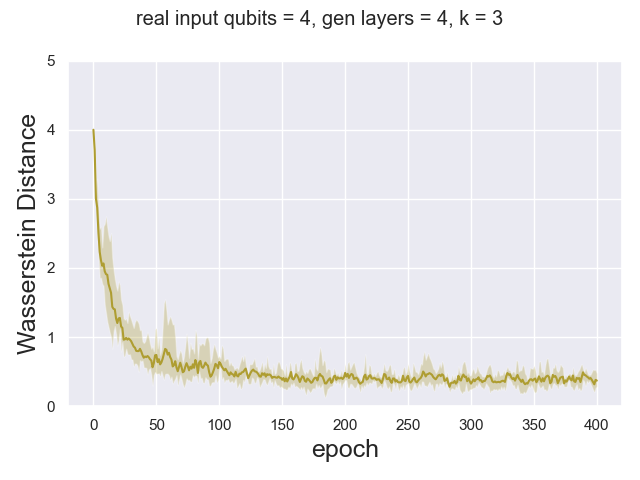
\includegraphics[width=0.3\linewidth]{figures/wqgans_phase_size=4_k=3_gen=4/Wasserstein_Distance.png}
  }
  \subfloat{
    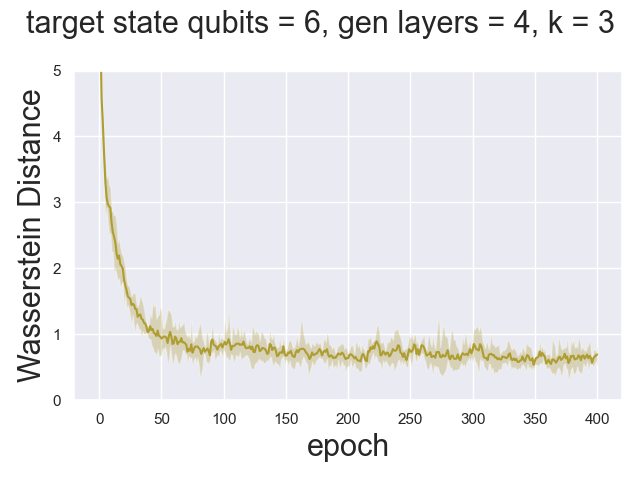
\includegraphics[width=0.3\linewidth]{figures/wqgans_phase_size=6_k=3_gen=4/Wasserstein_Distance.png}
  }
  \subfloat{
    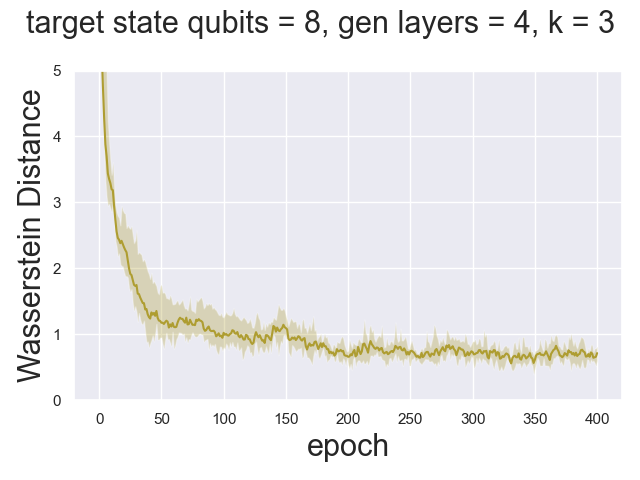
\includegraphics[width=0.3\linewidth]{figures/wqgans_phase_size=8_k=3_gen=4/Wasserstein_Distance.png}
  }

  \subfloat{
    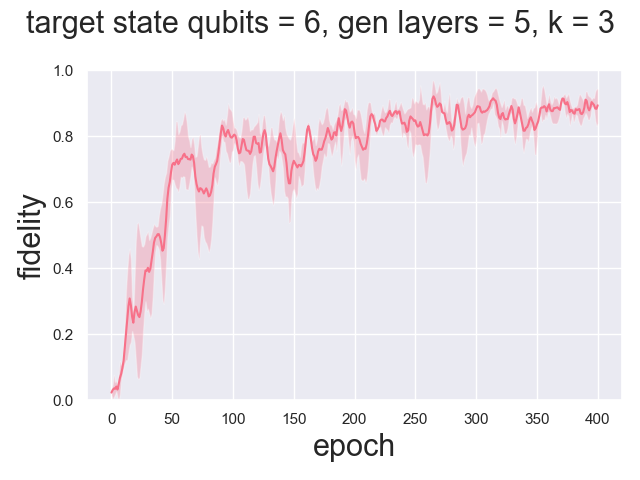
\includegraphics[width=0.3\linewidth]{figures/wqgans_phase_size=6_k=3_gen=5/fidelity.png}
  }
  \subfloat{
    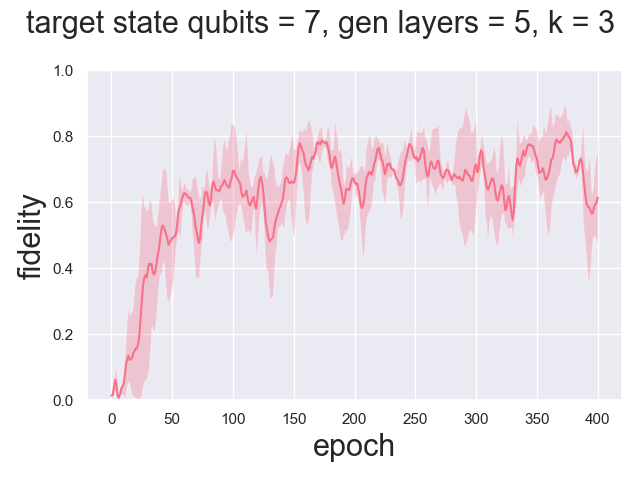
\includegraphics[width=0.3\linewidth]{figures/wqgans_phase_size=7_k=3_gen=5/fidelity.png}
  }
  \subfloat{
    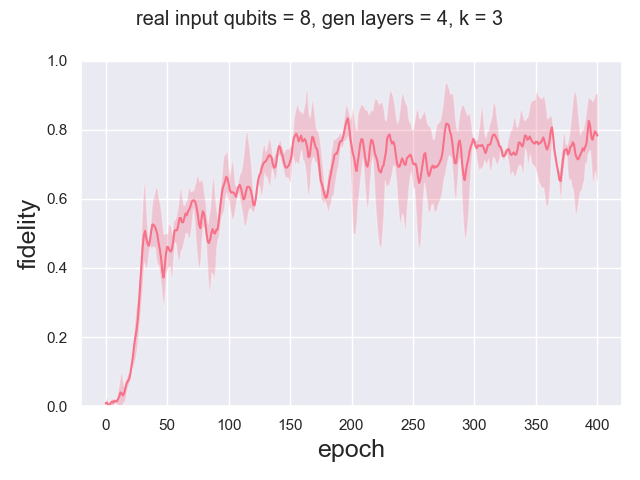
\includegraphics[width=0.3\linewidth]{figures/wqgans_phase_size=8_k=3_gen=5/fidelity.png}
  }

  \subfloat{
    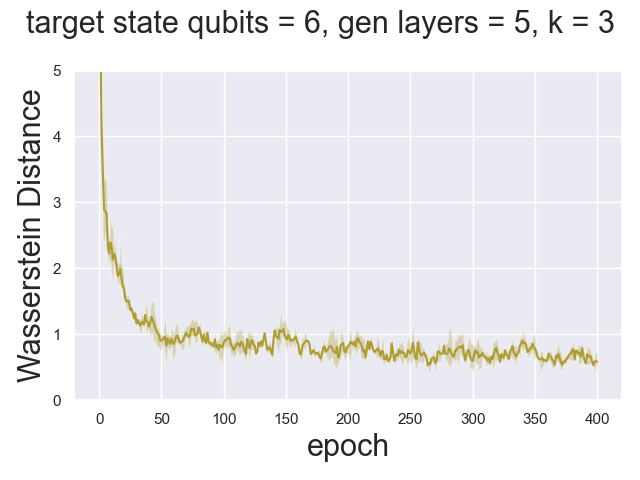
\includegraphics[width=0.3\linewidth]{figures/wqgans_phase_size=6_k=3_gen=5/Wasserstein_Distance.png}
  }
  \subfloat{
    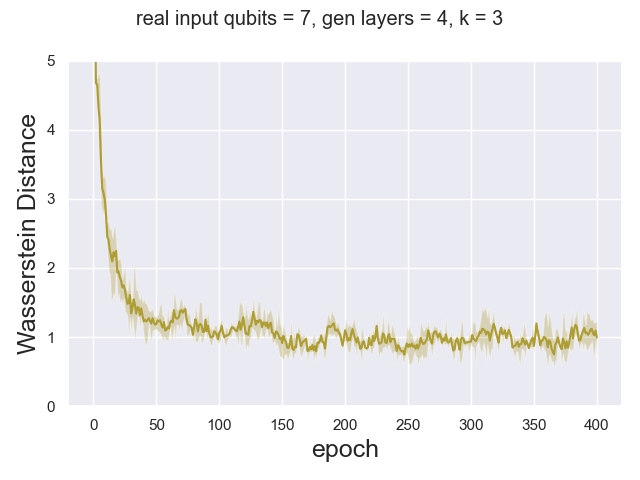
\includegraphics[width=0.3\linewidth]{figures/wqgans_phase_size=7_k=3_gen=5/Wasserstein_Distance.png}
  }
  \subfloat{
    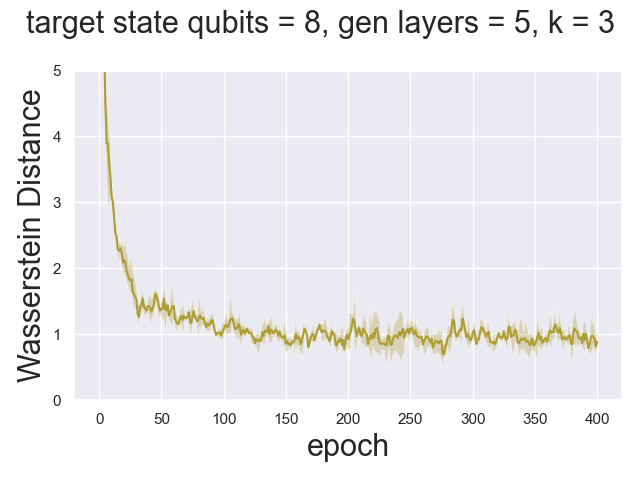
\includegraphics[width=0.3\linewidth]{figures/wqgans_phase_size=8_k=3_gen=5/Wasserstein_Distance.png}
  }
  \caption{Results for the target state generated with the topological phase
    transition circuit (Appendix \ref{apx:topological_phase_transition_ansatz})
    and the generator built with the generic circuit (Appendix \ref{apx:sqgans_ansatz}).
    The solid line represents the average value and the shaded area
    represents the range from 5 different experiments. First the
    fidelity is shown and below the corresponding Wasserstein distance.}
  \label{fig:wqgans_phase_res_3}
\end{figure}


\begin{figure}[htbp!]
  \captionsetup[subfigure]{labelformat=empty}
  \centering
  \subfloat{
    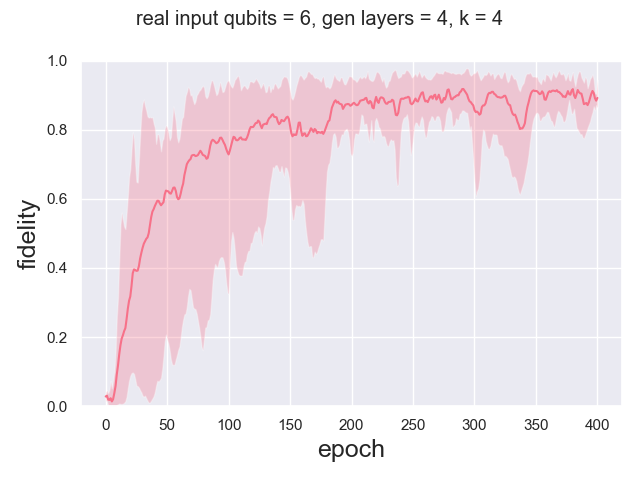
\includegraphics[width=0.3\linewidth]{figures/wqgans_phase_size=6_k=4_gen=4/fidelity.png}
  }
  \subfloat{
    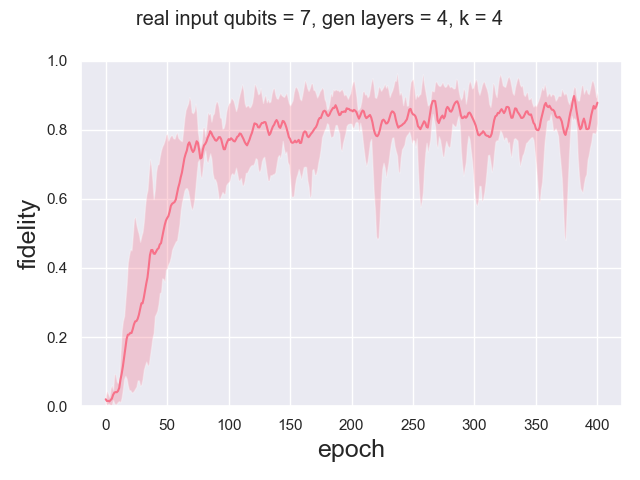
\includegraphics[width=0.3\linewidth]{figures/wqgans_phase_size=7_k=4_gen=4/fidelity.png}
  }
  \subfloat{
    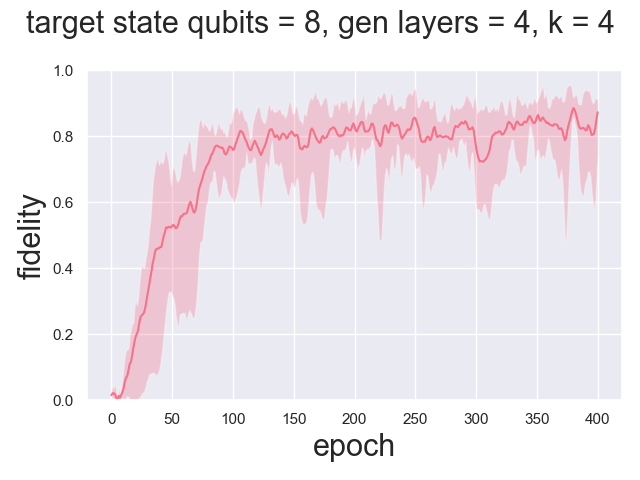
\includegraphics[width=0.3\linewidth]{figures/wqgans_phase_size=8_k=4_gen=4/fidelity.png}
  }

  \subfloat{
    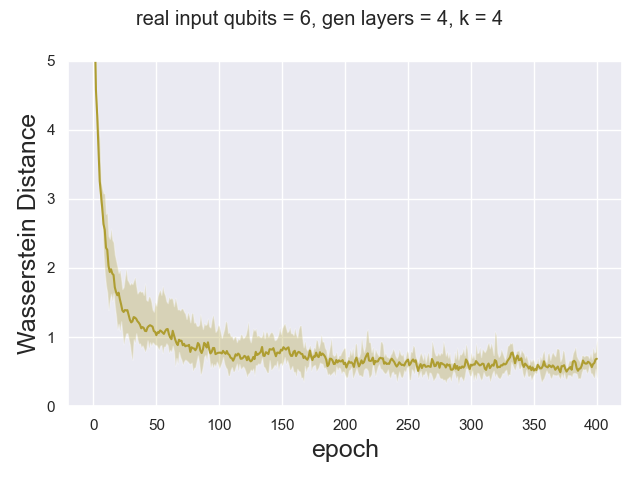
\includegraphics[width=0.3\linewidth]{figures/wqgans_phase_size=6_k=4_gen=4/Wasserstein_Distance.png}
  }
  \subfloat{
    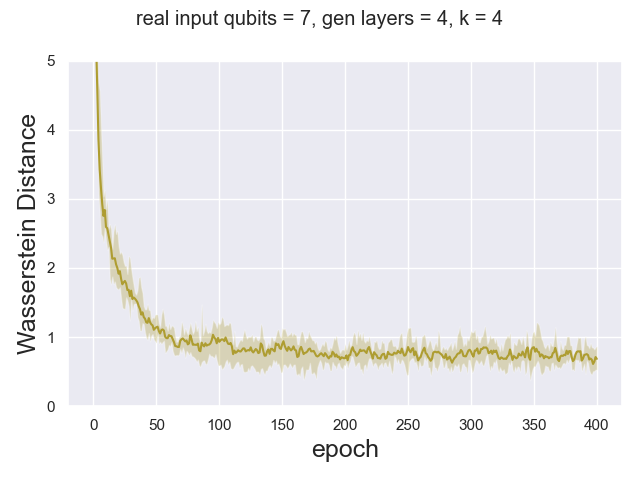
\includegraphics[width=0.3\linewidth]{figures/wqgans_phase_size=7_k=4_gen=4/Wasserstein_Distance.png}
  }
  \subfloat{
    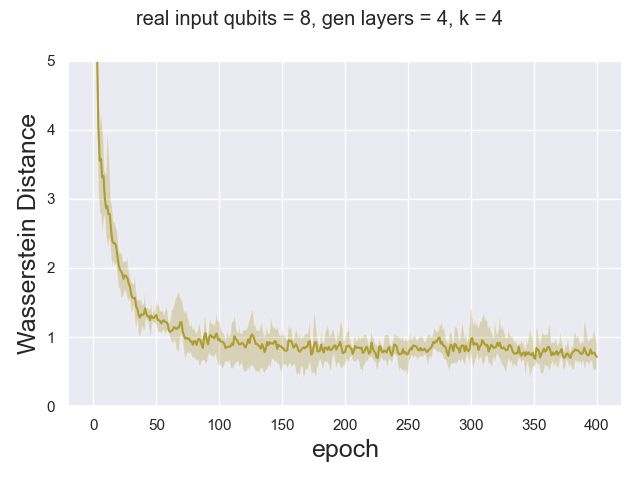
\includegraphics[width=0.3\linewidth]{figures/wqgans_phase_size=8_k=4_gen=4/Wasserstein_Distance.png}
  }
  
  \subfloat{
    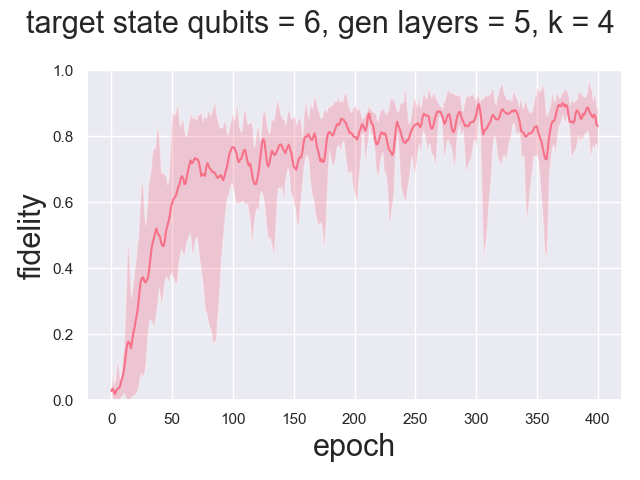
\includegraphics[width=0.3\linewidth]{figures/wqgans_phase_size=6_k=4_gen=5/fidelity.png}
  }
  \subfloat{
    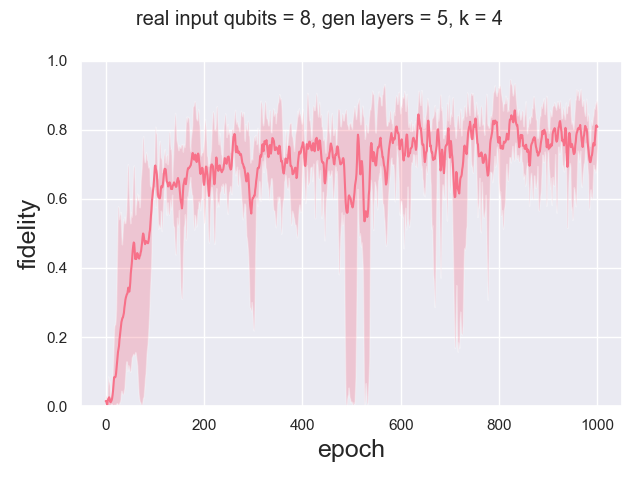
\includegraphics[width=0.3\linewidth]{figures/wqgans_phase_size=8_k=4_gen=5/fidelity.png}
  }
  \subfloat{
    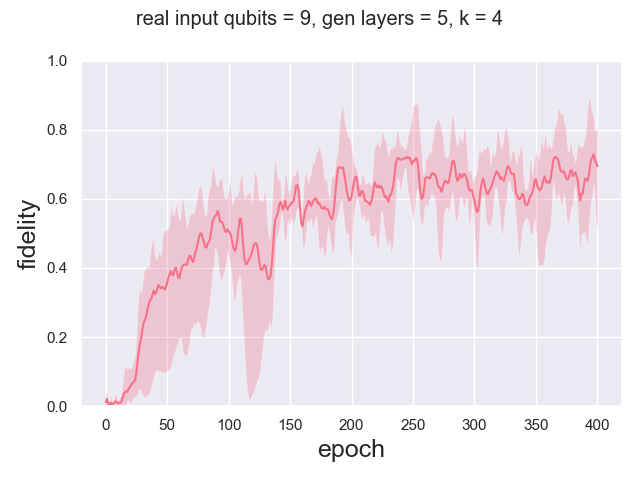
\includegraphics[width=0.3\linewidth]{figures/wqgans_phase_size=9_k=4_gen=5/fidelity.png}
  }

  \subfloat{
    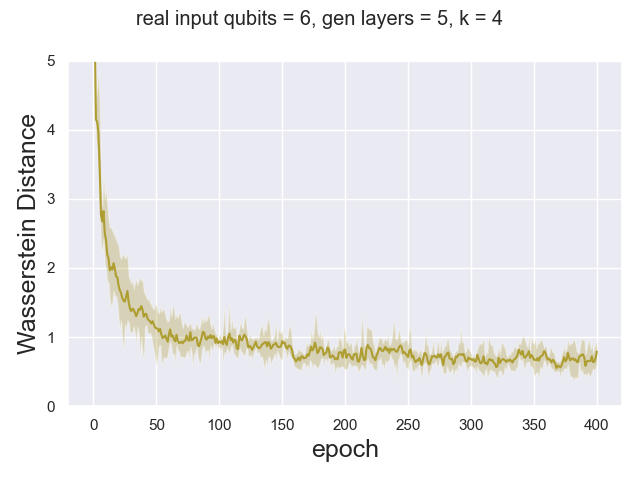
\includegraphics[width=0.3\linewidth]{figures/wqgans_phase_size=6_k=4_gen=5/Wasserstein_Distance.png}
  }
  \subfloat{
    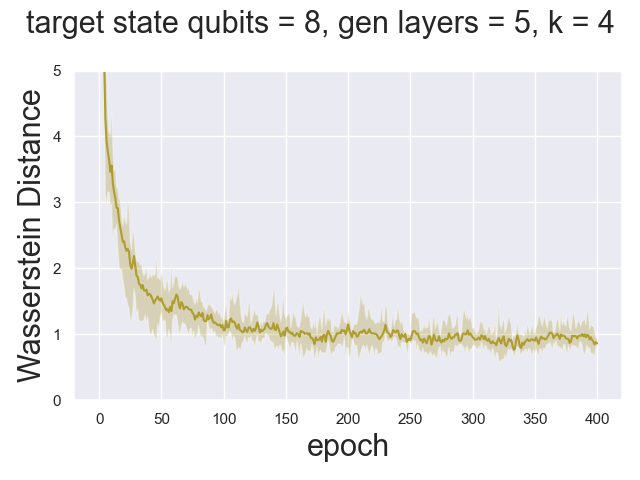
\includegraphics[width=0.3\linewidth]{figures/wqgans_phase_size=8_k=4_gen=5/Wasserstein_Distance.png}
  }
  \subfloat{
    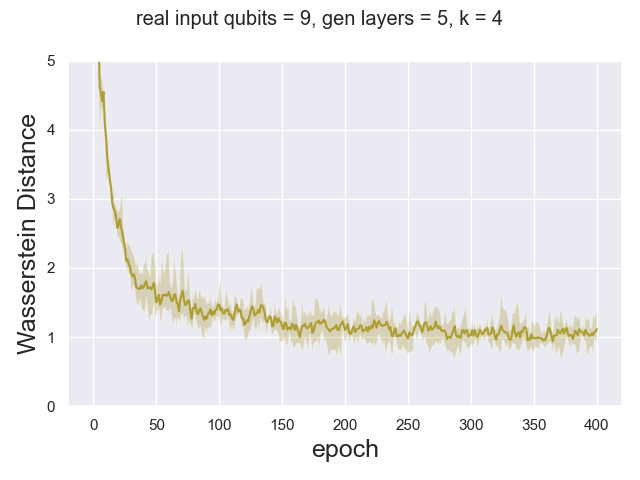
\includegraphics[width=0.3\linewidth]{figures/wqgans_phase_size=9_k=4_gen=5/Wasserstein_Distance.png}
  }
  \caption{
    Results for the target state generated with the topological phase
    transition circuit (Appendix \ref{apx:topological_phase_transition_ansatz})
    and the generator built with the generic circuit (Appendix \ref{apx:sqgans_ansatz}).
    The solid line represents the average value and the shaded area
    represents the range from 5 different experiments. First the
    fidelity is shown and below the corresponding Wasserstein distance.}
  \label{fig:wqgans_phase_res_5}
\end{figure}
\label{apx:wqgans_pahse_results_butterfly}

\begin{figure}[htbp!]
  \captionsetup[subfigure]{labelformat=empty}
  \centering
  \subfloat{
    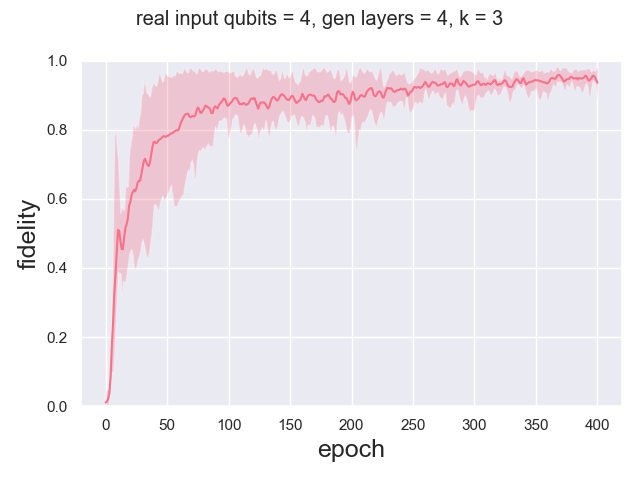
\includegraphics[width=0.25\linewidth]{figures/wqgans_butterfly_size=4_k=3_gen=4/fidelity.png}
  }
  \subfloat{
    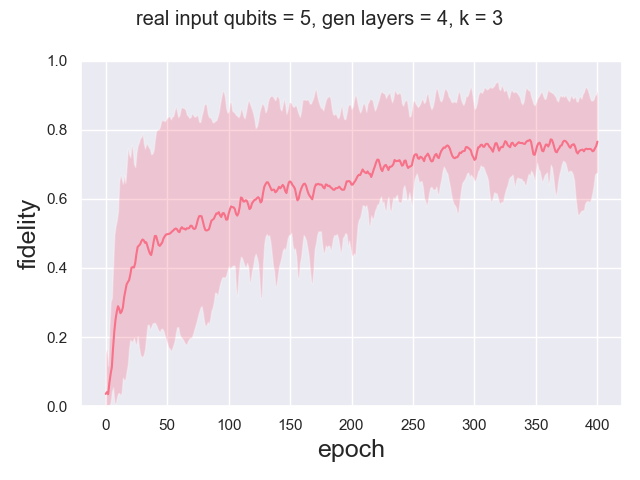
\includegraphics[width=0.25\linewidth]{figures/wqgans_butterfly_size=5_k=3_gen=4/fidelity.png}
  }
  \subfloat{
    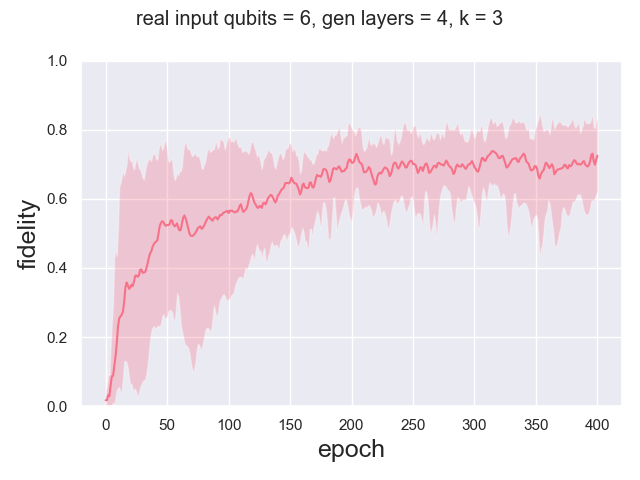
\includegraphics[width=0.25\linewidth]{figures/wqgans_butterfly_size=6_k=3_gen=4/fidelity.png}
  }
  \subfloat{
    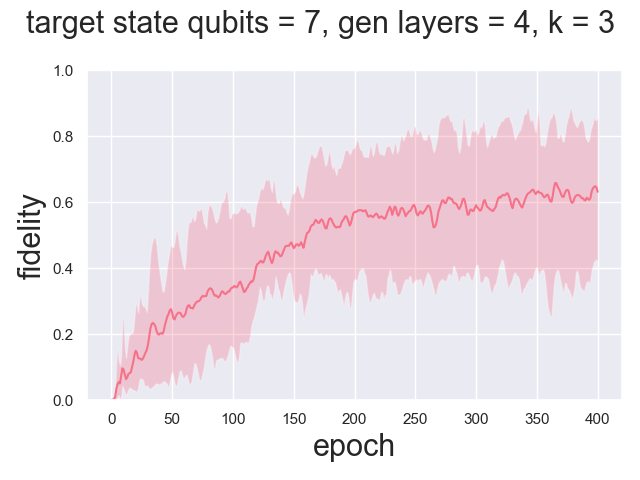
\includegraphics[width=0.25\linewidth]{figures/wqgans_butterfly_size=7_k=3_gen=4/fidelity.png}
  }

  \subfloat{
    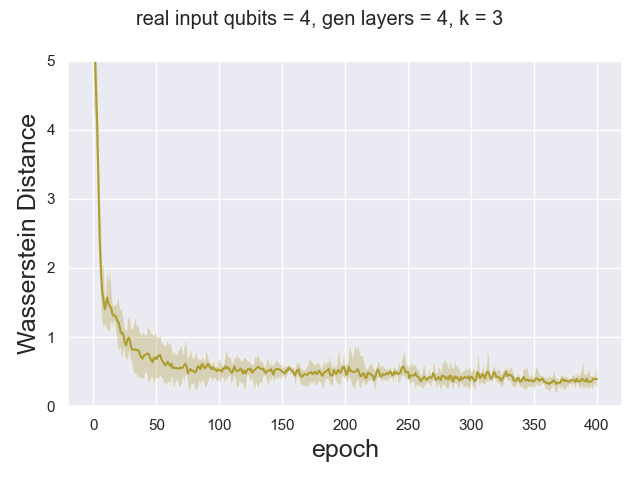
\includegraphics[width=0.25\linewidth]{figures/wqgans_butterfly_size=4_k=3_gen=4/Wasserstein_Distance.png}
  }
  \subfloat{
    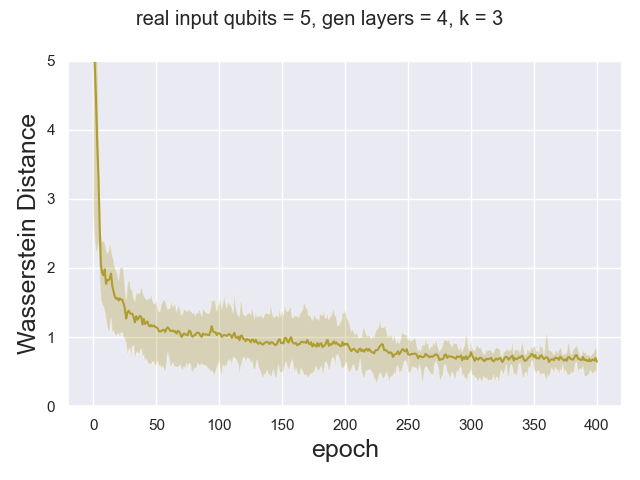
\includegraphics[width=0.25\linewidth]{figures/wqgans_butterfly_size=5_k=3_gen=4/Wasserstein_Distance.png}
  }
  \subfloat{
    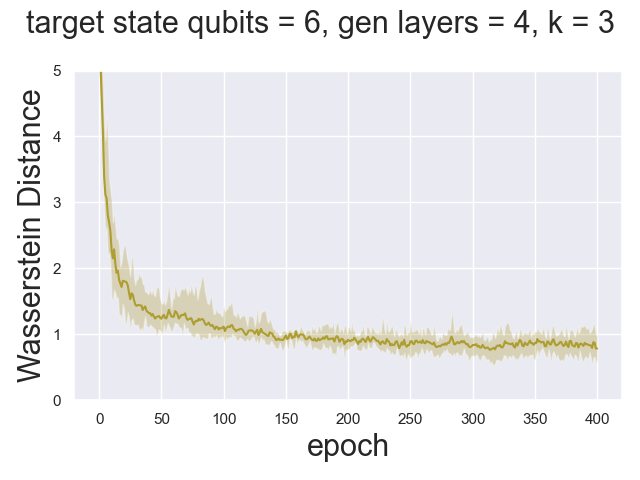
\includegraphics[width=0.25\linewidth]{figures/wqgans_butterfly_size=6_k=3_gen=4/Wasserstein_Distance.png}
  }
  \subfloat{
    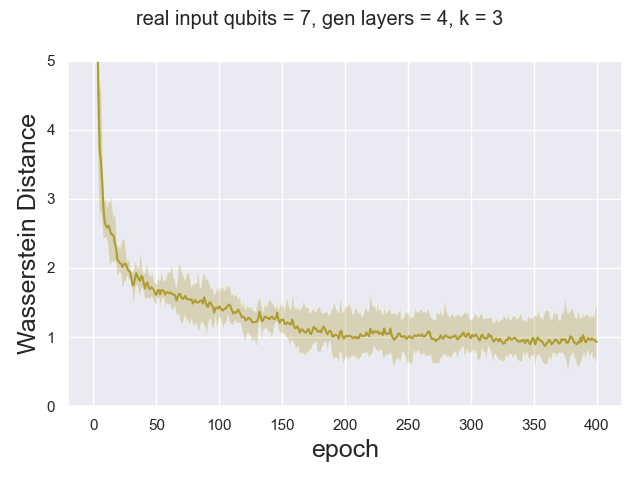
\includegraphics[width=0.25\linewidth]{figures/wqgans_butterfly_size=7_k=3_gen=4/Wasserstein_Distance.png}
  }

  \subfloat{
    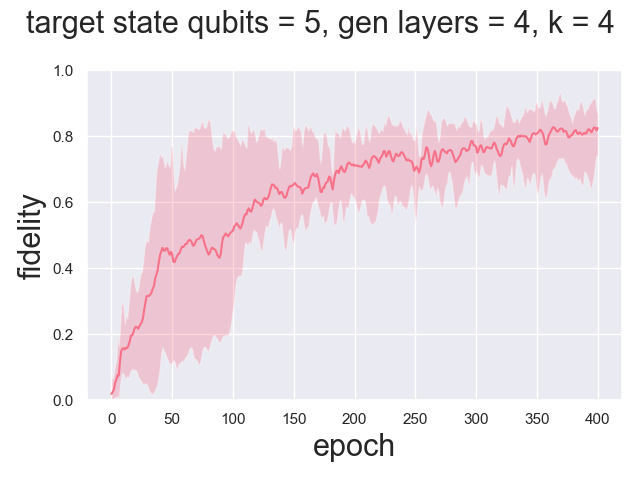
\includegraphics[width=0.25\linewidth]{figures/wqgans_butterfly_size=5_k=4_gen=4/fidelity.png}
  }
  \subfloat{
    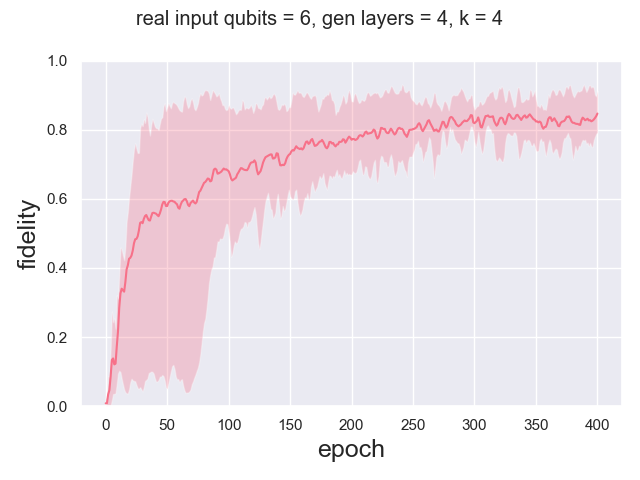
\includegraphics[width=0.25\linewidth]{figures/wqgans_butterfly_size=6_k=4_gen=4/fidelity.png}
  }
  \subfloat{
    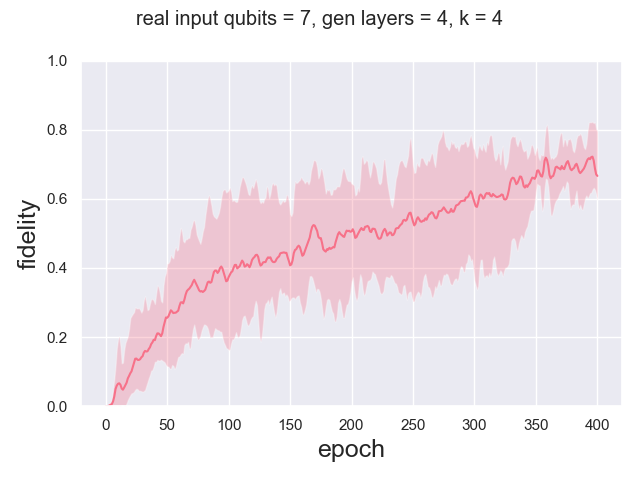
\includegraphics[width=0.25\linewidth]{figures/wqgans_butterfly_size=7_k=4_gen=4/fidelity.png}
  }
  \subfloat{
    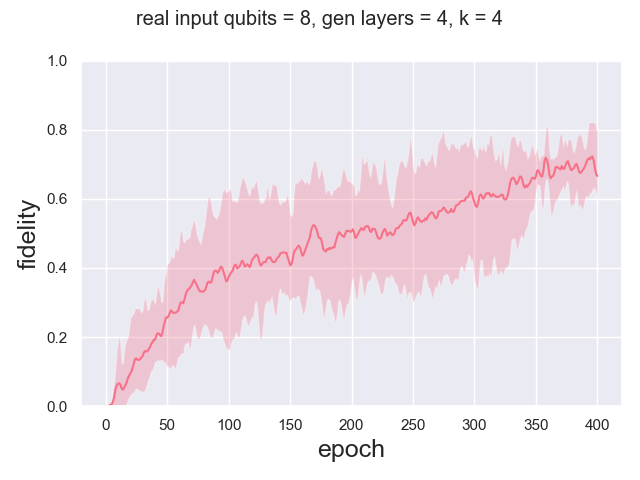
\includegraphics[width=0.25\linewidth]{figures/wqgans_butterfly_size=8_k=4_gen=4/fidelity.png}
  }

  \subfloat{
    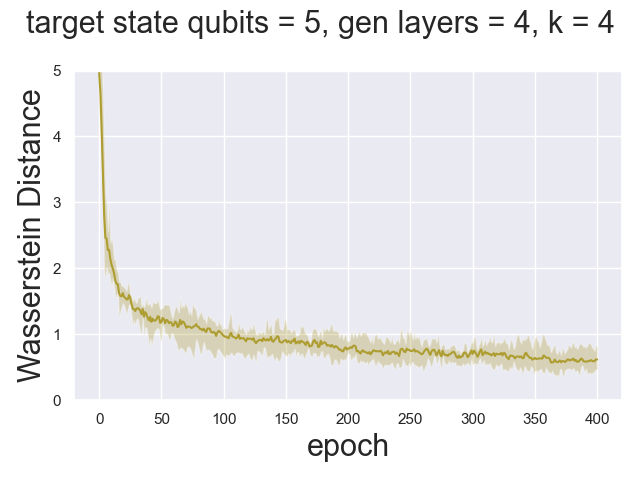
\includegraphics[width=0.25\linewidth]{figures/wqgans_butterfly_size=5_k=4_gen=4/Wasserstein_Distance.png}
  }
  \subfloat{
    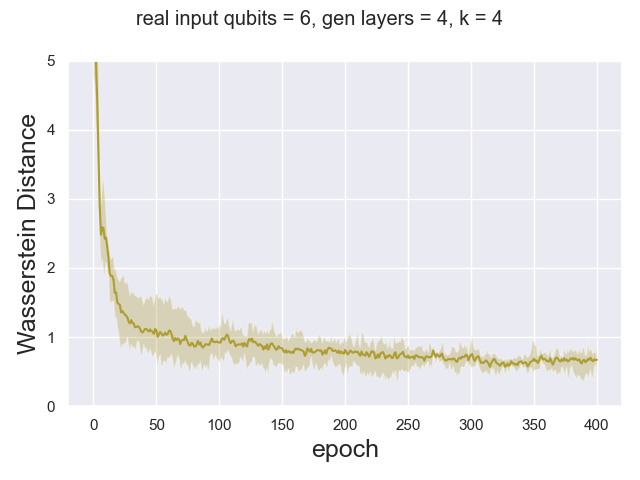
\includegraphics[width=0.25\linewidth]{figures/wqgans_butterfly_size=6_k=4_gen=4/Wasserstein_Distance.png}
  }
  \subfloat{
    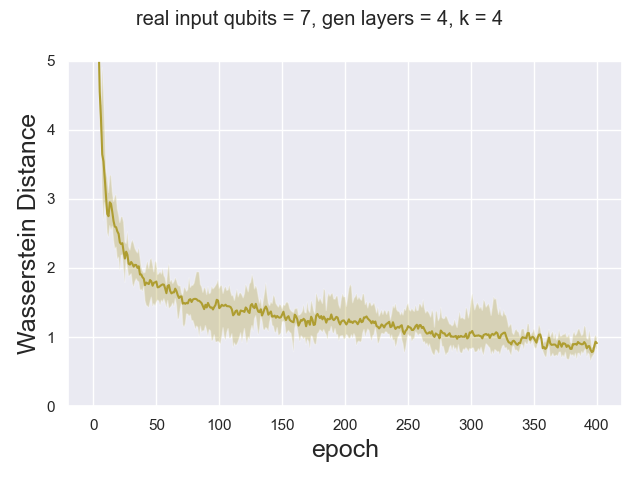
\includegraphics[width=0.25\linewidth]{figures/wqgans_butterfly_size=7_k=4_gen=4/Wasserstein_Distance.png}
  }
  \subfloat{
    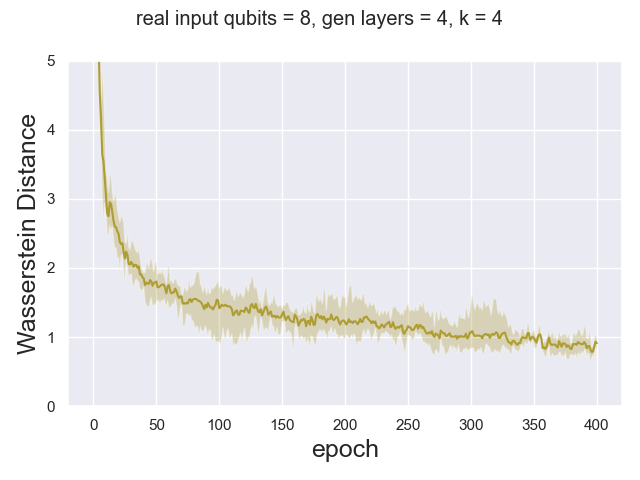
\includegraphics[width=0.25\linewidth]{figures/wqgans_butterfly_size=8_k=4_gen=4/Wasserstein_Distance.png}
  }
  \caption{Results for the target state generated with the butterfly circuit (Appendix \ref{apx:butterfly_ansatz})
    and the generator built with the generic circuit (Appendix \ref{apx:sqgans_ansatz}).
    The solid line represents the average value and the shaded area
    represents the range from 5 different experiments. First the
    fidelity is shown and below the corresponding Wasserstein distance.}
  \label{fig:wqgans_res_butterfly_3}
\end{figure}
\let\clearpage\oldclearpage
\chapter{Code and Technologies}
All the code used for this work is available on public github repository:
\url{https://github.com/WiktorJ/quantum-gans}.

The quantum circuits were implemented using Cirq
\cite{https://doi.org/10.5281/zenodo.5138274} and evaluated using Tensorflow
Quantum \cite{broughton2020tensorflow}. The optimization of the classical and
quantum networks was performed using optimizers from Tensorflow library \cite{tensorflow2015-whitepaper}.

All the quantum circuits schematics were drawn using Quantikz \cite{https://doi.org/10.17637/rh.7000520}.


% \section{Example 1}
% \cmark
% \section{Example 2}
% \xmark

%%% Local Variables:
%%% mode: latex
%%% TeX-master: "../main"
%%% End: